\documentclass[tikz,border=3pt]{standalone}

\usepackage[T1]{fontenc}
\usepackage{newtxtext,newtxmath}
\let\Bbbk\relax
\usepackage{amsmath,amssymb}
\usetikzlibrary{arrows.meta,calc}

\begin{document}

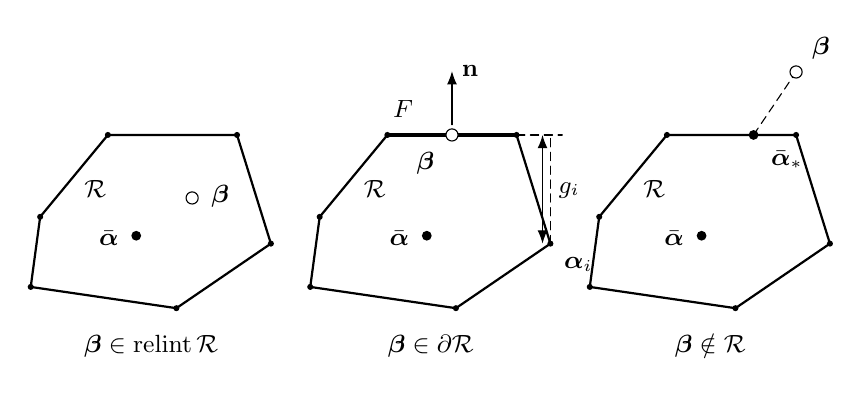
\begin{tikzpicture}[
  >=Latex,
  line cap=round,
  line join=round,
  every node/.style={font=\small},
  response/.style={circle,fill,inner sep=1.25pt},
  target/.style={circle,draw,fill=white,inner sep=1.55pt},
  hull/.style={thick},
  guide/.style={densely dashed}
]

% ------------------------------------------------------------------
% Interior supply
% ------------------------------------------------------------------
\begin{scope}[xshift=0cm]
  \coordinate (A1) at (0,0.45);
  \coordinate (A2) at (1.85,0.18);
  \coordinate (A3) at (3.05,1.00);
  \coordinate (A4) at (2.62,2.38);
  \coordinate (A5) at (0.98,2.38);
  \coordinate (A6) at (0.12,1.34);

  \draw[hull] (A1)--(A2)--(A3)--(A4)--(A5)--(A6)--cycle;
  \foreach \P in {A1,A2,A3,A4,A5,A6}
    \fill (\P) circle (1.1pt);

  \node at (0.82,1.70) {$\mathcal R$};

  \coordinate (r) at (1.34,1.10);
  \coordinate (y) at (2.05,1.58);
  \node[response] at (r) {};
  \node[anchor=east] at ($(r)+(-0.10,-0.03)$) {$\bar{\boldsymbol\alpha}$};
  \node[target] at (y) {};
  \node[anchor=west] at ($(y)+(0.12,0.02)$) {$\boldsymbol\beta$};

  \node at (1.53,-0.30) {$\boldsymbol\beta\in\operatorname{relint}\mathcal R$};
\end{scope}

% ------------------------------------------------------------------
% Boundary supply
% ------------------------------------------------------------------
\begin{scope}[xshift=3.55cm]
  \coordinate (B1) at (0,0.45);
  \coordinate (B2) at (1.85,0.18);
  \coordinate (B3) at (3.05,1.00);
  \coordinate (B4) at (2.62,2.38);
  \coordinate (B5) at (0.98,2.38);
  \coordinate (B6) at (0.12,1.34);

  \draw[hull] (B1)--(B2)--(B3)--(B4)--(B5)--(B6)--cycle;
  \foreach \P in {B1,B2,B3,B4,B5,B6}
    \fill (\P) circle (1.1pt);

  \node at (0.82,1.70) {$\mathcal R$};

  \draw[line width=1.4pt] (B5)--(B4);
  \node[anchor=south] at (1.18,2.48) {$F$};

  \coordinate (r) at (1.48,1.10);
  \coordinate (y) at (1.80,2.38);
  \node[response] at (r) {};
  \node[anchor=east] at ($(r)+(-0.10,-0.03)$) {$\bar{\boldsymbol\alpha}$};
  \node[target] at (y) {};
  \node[anchor=north east] at ($(y)+(-0.10,-0.10)$) {$\boldsymbol\beta$};

  \draw[->] ($(y)+(0,0.13)$) -- ++(0,0.68) node[anchor=west] {$\mathbf n$};

  \coordinate (ai) at (3.05,1.00);
  \coordinate (proj) at (3.05,2.38);
  \draw[guide] (B4)--(3.20,2.38);
  \draw[guide] (ai)--(proj);
  \draw[<->] ($(ai)+(-0.10,0)$)--($(proj)+(-0.10,0)$);
  \node[anchor=west] at (3.03,1.68) {$g_i$};
  \node[anchor=north west] at ($(ai)+(0.05,-0.05)$) {$\boldsymbol\alpha_i$};

  \node at (1.53,-0.30) {$\boldsymbol\beta\in\partial\mathcal R$};
\end{scope}

% ------------------------------------------------------------------
% Exterior supply
% ------------------------------------------------------------------
\begin{scope}[xshift=7.10cm]
  \coordinate (C1) at (0,0.45);
  \coordinate (C2) at (1.85,0.18);
  \coordinate (C3) at (3.05,1.00);
  \coordinate (C4) at (2.62,2.38);
  \coordinate (C5) at (0.98,2.38);
  \coordinate (C6) at (0.12,1.34);

  \draw[hull] (C1)--(C2)--(C3)--(C4)--(C5)--(C6)--cycle;
  \foreach \P in {C1,C2,C3,C4,C5,C6}
    \fill (\P) circle (1.1pt);

  \node at (0.82,1.70) {$\mathcal R$};

  \coordinate (r) at (1.42,1.10);
  \coordinate (rs) at (2.08,2.38);
  \coordinate (y) at (2.62,3.18);

  \node[response] at (r) {};
  \node[anchor=east] at ($(r)+(-0.10,-0.03)$) {$\bar{\boldsymbol\alpha}$};
  \node[response] at (rs) {};
  \node[anchor=north west] at ($(rs)+(0.10,-0.08)$) {$\bar{\boldsymbol\alpha}_*$};

  \draw[guide] (rs)--(y);

  \node[target] at (y) {};
  \node[anchor=south west] at ($(y)+(0.08,0.04)$) {$\boldsymbol\beta$};

  \node at (1.53,-0.30) {$\boldsymbol\beta\notin\mathcal R$};
\end{scope}

\end{tikzpicture}

\end{document}
